


\section{Mapping irregular surfaces with an Accelerometer}
\begin{description}
\item[Hypotheses 1] : Vibrations of the Rollator increase while walking on surfaces with more hindrance. 
\item[Hypothesis 2] : The vibrations caused by the hindrance can be measured with the variance in the z-axis acceleration. 
\end{description}

Several test were conducted with the Measurement Rollator on different surfaces. Used the Accelerometer (Physics Toolbox version 1.3.7) and the Garmin to record GPS. The goal was to walk with an average walking speed of 4.7 km/h (3.2 – 6.2 km/h). This is the walking speed found from literature and own research. Though, while walking it felt quite fast. So the walking speed was kept around 4 km/h as best as possible. The researcher walked herself with the rollator over different surfaces. Each a distance of around 20 m. 

\subsubsection{Set-up}
The smart phone will always be placed horizontally on the Rollator. This means the z-axis is pointing down, and will correlate most with movements up and down. The x-axis will be pointing sideways and the y-axis front and back. Acceleration of walking speed will be seen in the y-axis. While turns will be seen in the x-axis. See figure ~\ref{setup} and ~\ref{setup2}

\begin{figure}[h]
\includegraphics[width=0.5\textwidth]{img/M_rollator_setup.pdf}
\centering
\caption{ Graphical representation of the direction of the axis of the accelerometer on the rollator. \label{setup}}
\end{figure}

\begin{figure}[h]
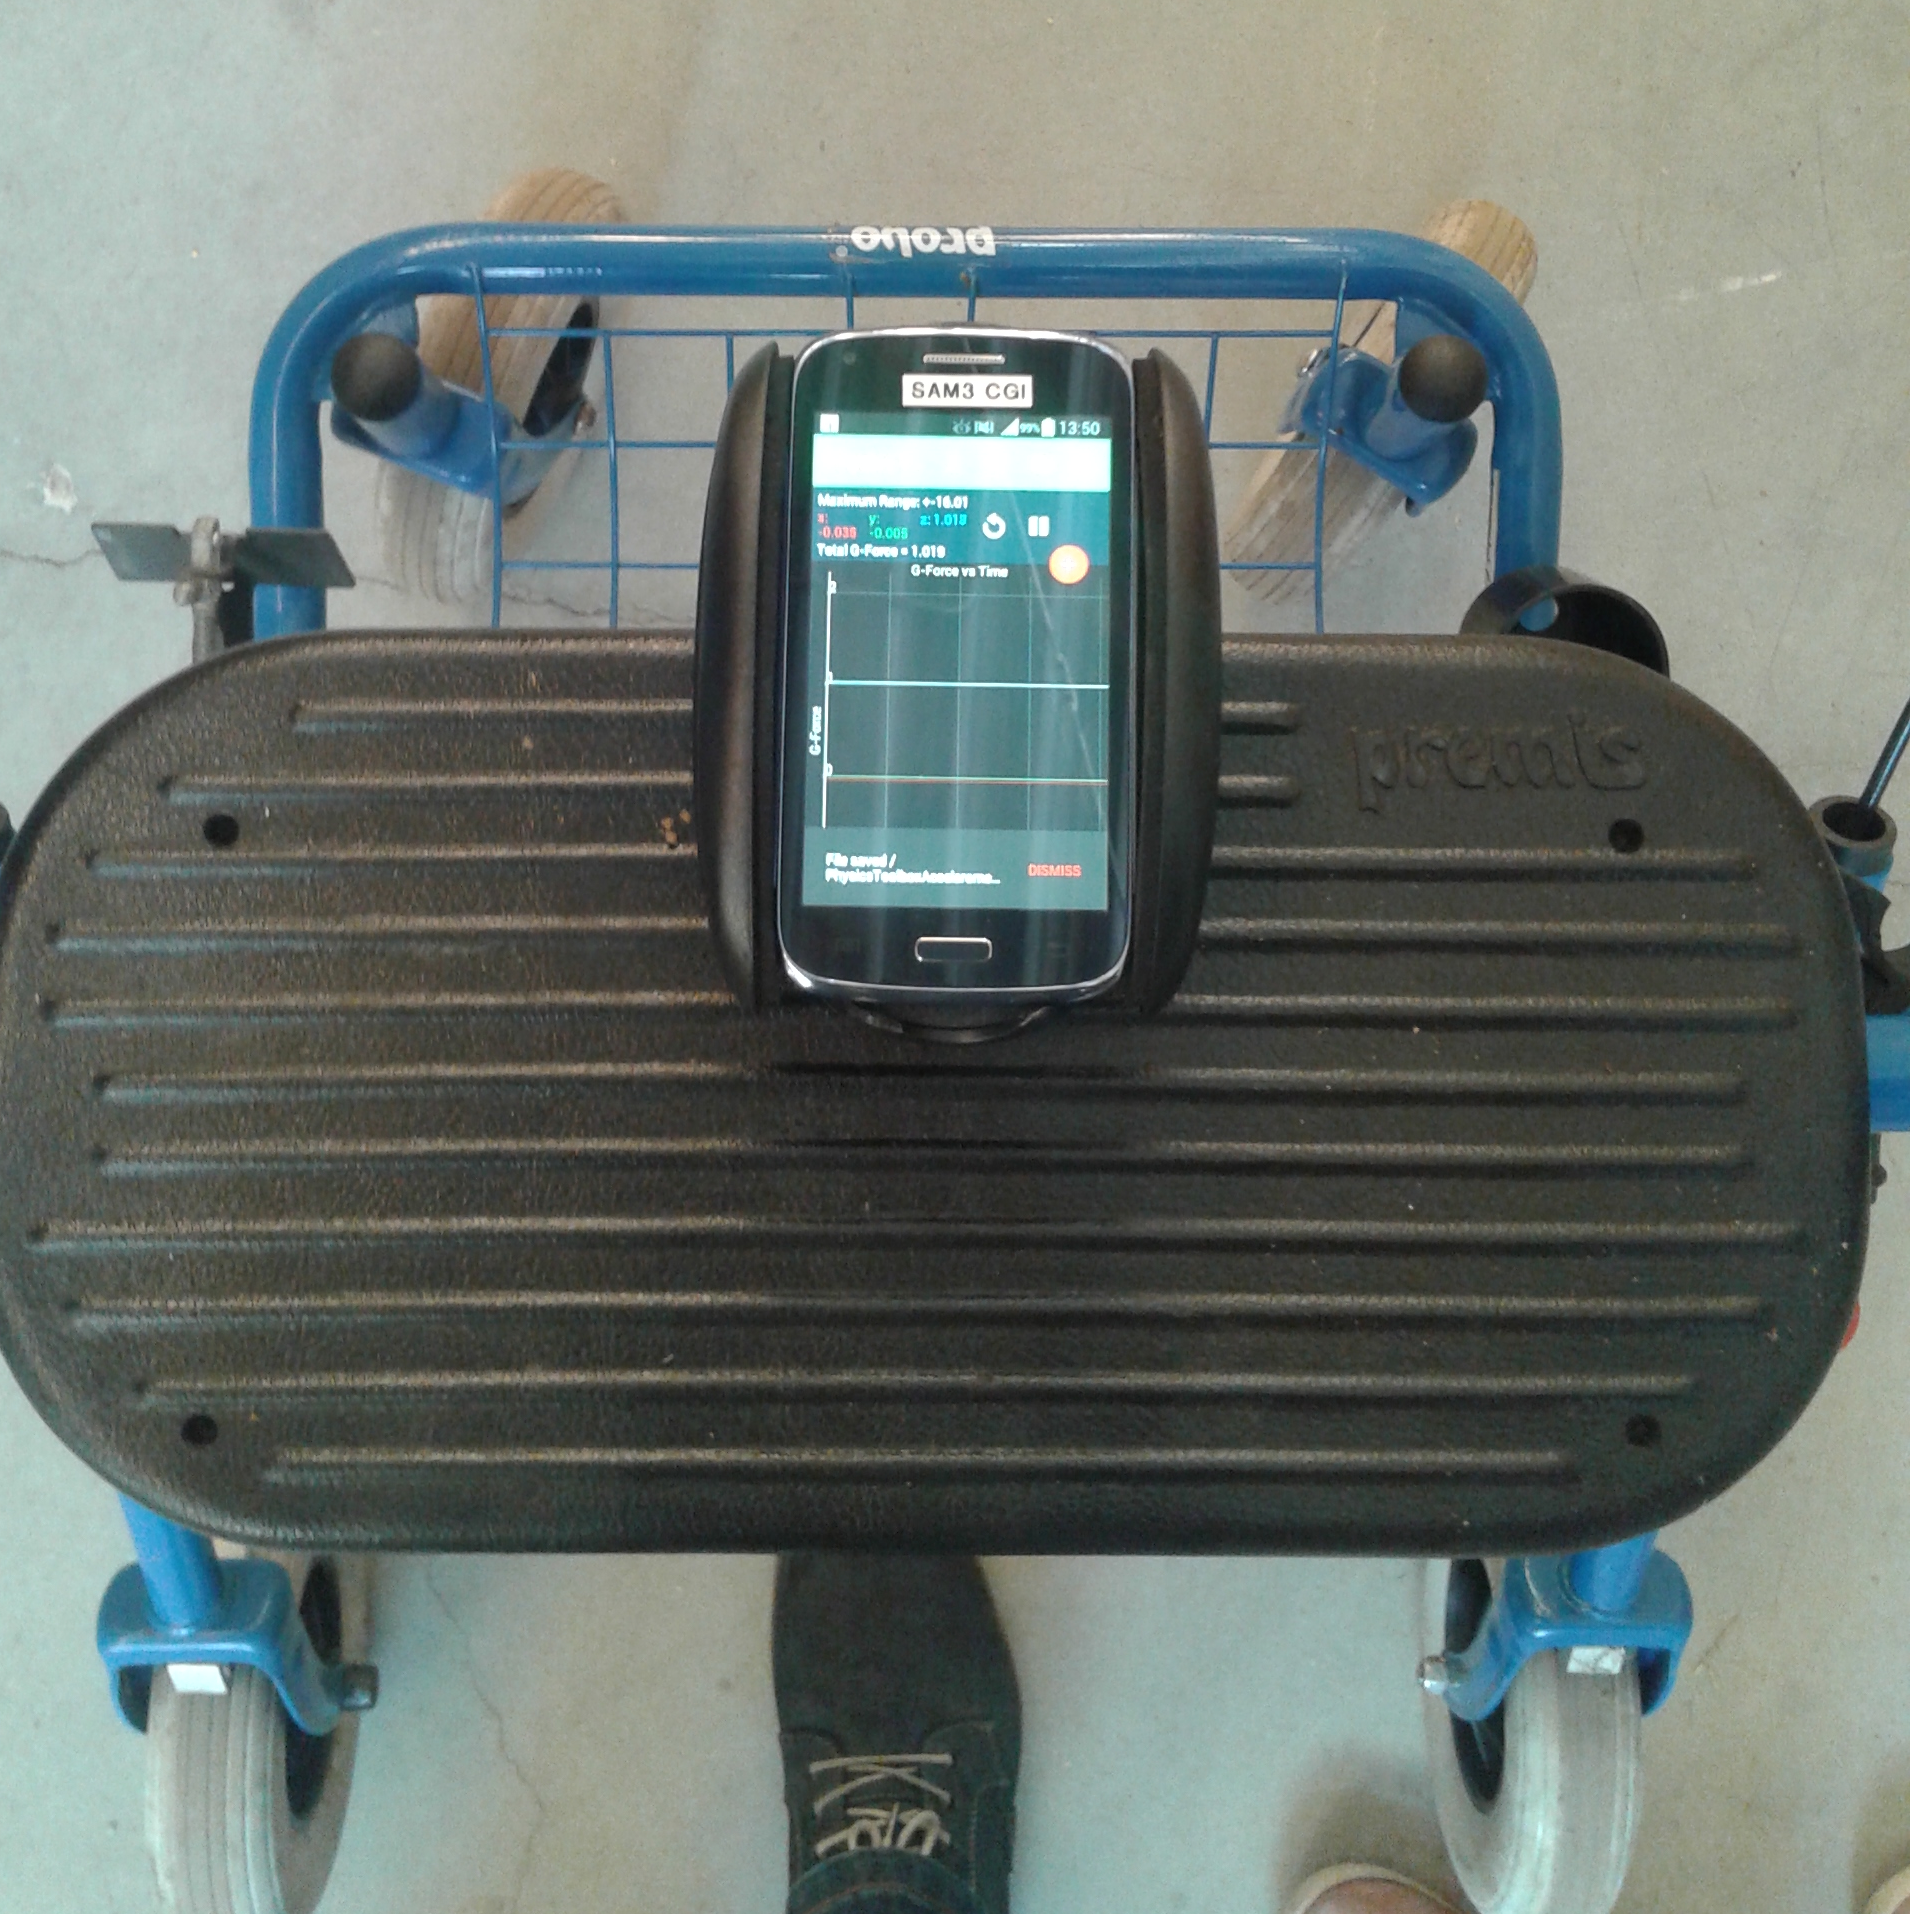
\includegraphics[width=0.5\textwidth]{img/M_setup}
\centering
\caption{ Set-up of smart phone attached to the measurement Rollator. \label{setup2}}
\end{figure}

All the pavement surfaces structures shown in image ~\ref{surfaceimg} were tested. Asphalt or tarmac, brick paving, tiles, gravel and grass. Also a smooth concrete surface inside was measured. 

\begin{figure}[h]
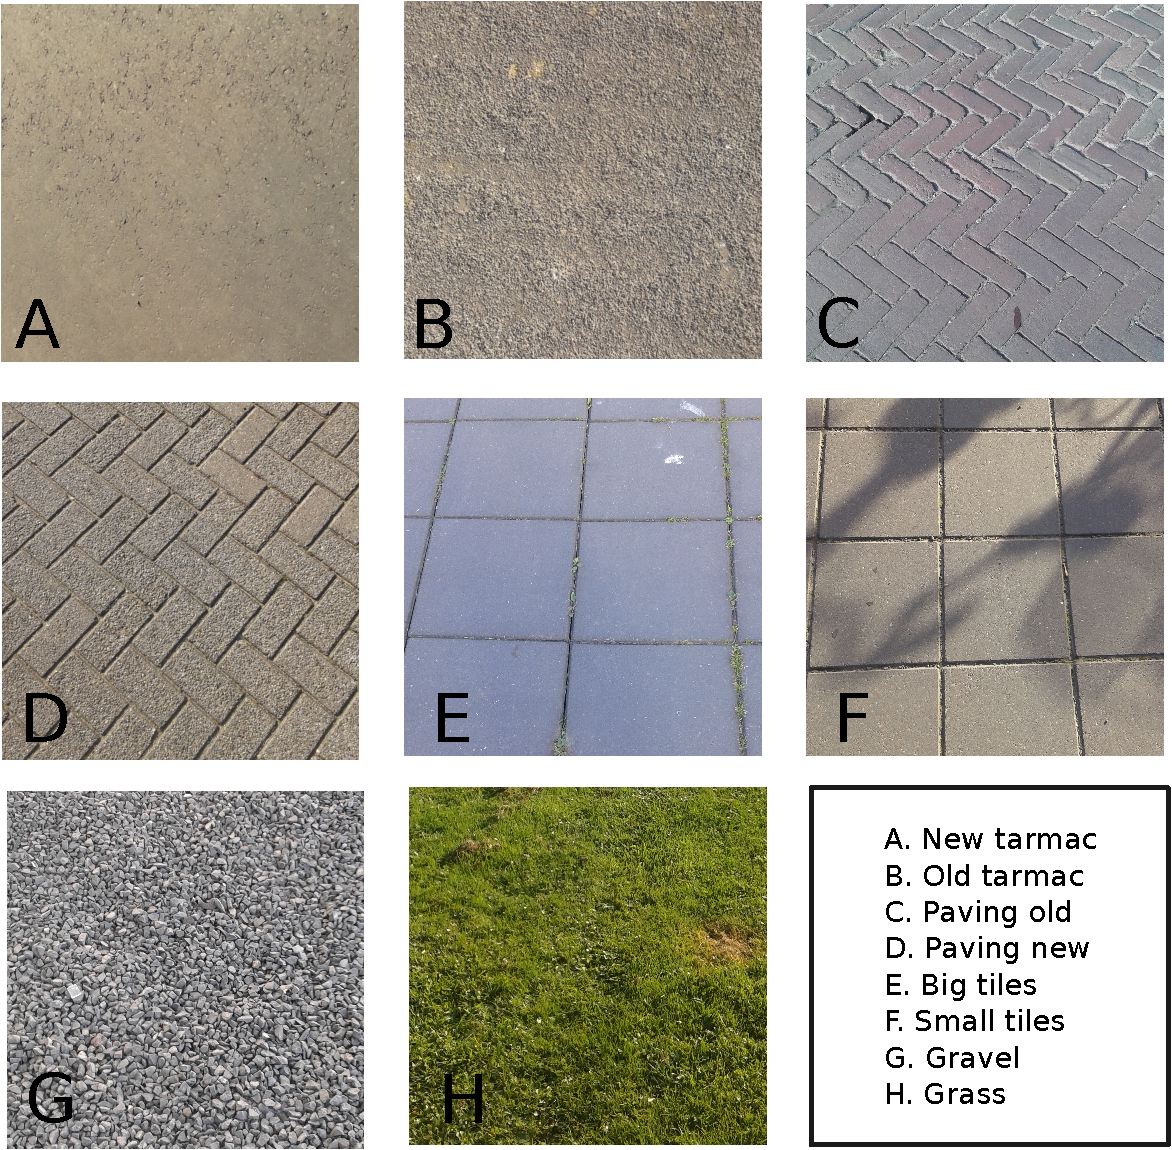
\includegraphics[width=0.7\textwidth]{img/M_all_surfaces}
\centering
\caption{Image of every measured surface \label{surfaceimg}}
\end{figure}
\clearpage

\subsection{Statistics}
By providing the descriptive statistics of the accelerometer output as a normal distribution, the differences in the vibrations on different surfaces can be explained. The data is approaching a normal distribution as can be seen in the example histogram or tarmac.(~\ref{hist})
\begin{figure}[!h]
\includegraphics[width=0.5\textwidth]{img/M_hist_tarmac_old.pdf}
\centering
\caption{Histogram of tarmac surface z-ax acceleration \label{hist}}
\end{figure}

Vibration goes into both directions so the mean will not show a surface specific outcome and will not differ much between the different surfaces. The means calculated only gave values around the 1. See table~\ref{stathindrance}.
% 4.3 statistic summary surface hindrance in results

The variability shows better how rouch the surface is. Therefore the variability is used, or the standard deviation together with the 5-number summary to create box plots. Including, the minimum, maximum, median and first and third quantile. To show a better understanding of the effect of the surface on the vibrations on the rollator. The formula for the mean variance and standard deviation:

\textbf{Mean:}  
\begin{equation}
Mean A_{z} = \frac{\sum_{k=1}^n A_{z}}{n}
\end{equation}

\textbf{Variance:}
\begin{equation}
\sigma^2 = \frac{\sum_{k=1}^n (A_{z}- mean(A_{z}))^2}{n-1}
\end{equation}

\textbf{Standard deviation:}
\begin{equation}
\sigma = \sqrt \frac{\sum_{k=1}^n (A_{z}- mean(A_{z}))^2}{n-1}
\end{equation}

\subsection{Comparison with Matthews et al. (2003)}
In Matthews et al. (2003)~\cite{Matthews2003} a reference score for hindrance of specific surfaces is provided. Shown in table~\ref{hindrance}. These values will be used as a reference, to see if the measured vibrations of the Accelerometer correlate. Because the reference numbers are relative, also the measured outcome is recalculated to a relative factor. Taking the most smooth surface as factor 1 and calculating the rest of the surfaces from this. See results in figure~\ref{comparefig} for a comparison of the values of Matthews and the calculated factors. 
 % figure comparison factors measured and given 4.3

\begin{table}[h]
\caption[Relative hindrance scores of surfaces]{Relative hindrance scores of surfaces, low scores represent levels of least hindrance ~\cite{Matthews2003} \label{hindrance}}
\centering
\begin{tabular}{|l|l|l|l|l|l|}
	\hline
	Concrete & Paving & Tarmac & Brick & Grass & Gravel\\
	\hline
	1 & 1.2 & 1.3 & 1.6 & 6 & 8 \\
	\hline
\end{tabular}
\end{table}

\section{Mapping abnormal or change events with change point detection using Accelerometer, GPS and AHN2 data}

Assuming that in the optimal circumstances, someone will walk with a specific speed in a monotonous way. Then, an \emph{abnormal} event in continuous data will indicate a problem or obstacle. 

\begin{description}
\item[Hypotheses 1] : Obstacles, curbs or bumps cause a sudden change in the walking behaviour and so can be seen by analysing the accelerometer and GPS time series and filtering out abnormal events in the time series.  
\item[Criteria]: 
\begin{itemize}
\item Sudden drop in speed.
\item Large change in all 3 axis of accelerometer or total acceleration. 
\item Sudden increase or change in slope or curvature. 
\end{itemize}
\end{description}

Going from one kind of surface to another will show a change in the vibrations. Also walking over a bump will show an abnormal peak in the measured acceleration. These changes in the vibrations of the axes can be determined by the change-point package of R containing specialized change-point finding algorithms for detecting multiple change-points within data and a variety of test statistics.~\cite{changepoint2015,  killick2014} 

The package contains functions to detect changes in the mean or the variance of the data. A change point is the estimation of the point at which the statistical properties of a sequence of observations changes. Having an ordered sequence of data $y_{1:n} = (y_{1}, .... , y_{n})$, a change-point is said to occur within this set when there exists a time, $τ ∈ {1, . . . , n − 1}$,such that the statistical properties of segment ${y_{1}, .... , y_{τ}}$ and segment ${y_{τ+1}, .... , y_{n}}$ are different in some way. Consequently the $m$ change-points will split the data into $m + 1$ segments, with the $i$th segment containing data $y_{(τ_{i−1} +1):τ_{i}}$ . Each segment will be summarized by a set of parameters.~\cite{killick2014}

% changing $y$ to $f$ for better distinction between y ax and data range ?



The changepoint package implements three multiple change-point algorithms; Binary Segmentation, Segment Neighbourhoods and the exact linear time, PELT. Binary Segmentation is an approximate algorithm and most widely used search method. Segment Neighbourhoods has a long computation time but is more exact. PELT is computationally fast and exact. The number of change-points increases linearly as the data set increases. The exact approach of identifying multiple change-points, formulas, methods and references can be found in~\cite{killick2014}

	
For this research the 2 sides of the change points are used; the change-points $CP_{1:m} = (CP_{1}, .... , CP_{m})$ themselves and the segments $y_{(CP_{i−1} +1):CP_{i}}$ between the change-points, eacht, with its set of parameters. For the vibrations measured by the accelerometer, the change-points indicate an abnormal event while the segments between the change-points indicate a phase of monotonous movement or monotonous surface. 


For the accelerometer data always has the mean around the same number, the degree of hindrance or occurrence of an obstacle, will show more in the variance of the data. 


The changes are detected using the exact multiple change-point method (PELT or SegNeigh) or approximate (BinSeg) methods. ~\cite{changepoint2015}\newline

For testing if the change-point method is usable for detecting obstacles while walking, a bike ride was monitored and a walk with the measurement rollator. 
Several more test were walked, during the RollatorLoop 2015, but these measurements failed. See Annex \ref{} for the measured tracks and the accelerometer output. 

The tracks measured with the geoTracker application and the Accelerometer application on the smart phone which did succeeded are shown in figure \ref{tracks}. 

\begin{figure}[h]
\includegraphics[width=\textwidth]{img/M_map_routes.pdf}
\centering
\caption{ Map of both tracks used \label{tracks}}
\end{figure}

\subsection{Segments between changepoints}
The average variance of the segment indicates the surface characteristics. If combined with the location, the values indicate characteristics of the walk and walk changes. Even the location specific characteristics can be extracted to the time-series observations.

The feature vector for every $ith$  observation for the 3-axis signal is represented by:

\begin{equation}
F_{xyz}(i) = [ x, y, z, A_{m}, Var(A_{z}), Var(A_{m})]  %% and all other stuff needed. 
\end{equation}

To this we could add the average variance per segment between the change-points:

\begin{equation}
F_{xyz}(seg) = [Var(A_{z}), Var(A_{m})]
\end{equation}

For reference, the change-points are linked to the location by using the time-stamp of the accelerometer and the GPS points. With the time stamp, the first GPS point before and the first GPS point after that time is taken. Because the time difference between the first GPS point and the change point is known and the speed between the GPS points $(s)$, the distance and so location of the change point is calculated. 

\begin{figure}[h]
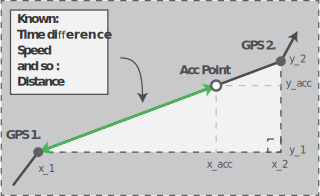
\includegraphics[width=0.75\textwidth]{img/M_location_calc.pdf}
\centering
\caption{Graphical explanation of change point location calculations \label{cpcalc}}
\end{figure}

With coordinates ($x_{1}, y_{1}$) and  ($x_{2}, y_{2}$) in RDnew as the known first and second GPS point, respectively. 

Distance between $(x_{1}, y_{1})(x_{2}, y_{2})$:
\begin{equation}
d_{1,2} = \sqrt (y_{1}-y_{2})^2 + (x_{1}-x_{2})^2 
\end{equation}

Distance between $(x_{1}, y_{1})(x_{cp}, y_{cp})$:
\begin{equation}
d_{1,cp} = s * time difference((x_{1}, y_{1}) - (x_{cp}, y_{cp}))
\end{equation}

New $x$ coordinate:
\begin{equation}
x_{cp} = x_{1} +  \frac{d_{1,cp}}{d_{1,2}} * (x_{2} - x_{1})
\end{equation}

New $y$ coordinate:
\begin{equation}
y_{cp} = y_{1} +  \frac{d_{1,cp}}{d_{1,2}} * (y_{2} - y_{1})
\end{equation}


Now we can also add the location specific data to the accelerometer segments, the speed($S$) extracted from the track GPS points and the AHN values, height, slope and curvature. Resulting in a feature per observation of:


\begin{multline} 
\centering
	\begin{equation*} F_{xyz}(i) = \end{equation*}
	\\
	\begin{equation*}[ A_{x}, A_{y}, A_{z}, A_{m}, Var(A_{z}), Var(A_{m}), \end{equation*}
	\\
	\begin{equation} Var(A_{z seg}), Var(A_{mseg}) , s, height, slope, curvature ] \end{equation}
\end{multline}

And the average values for the segments between the change-points:

\begin{equation} 
F_{xyz}(seg) = [ Var(A_{z}), Var(A_{m}), Var(A_{z seg}), Var(A_{mseg}) , A_s, A_height, A_slope, A_curvature ] 
\end{equation}

With cross correlation between the several features, we can detect which feature best represents the walk characteristics. 

By doing a cross correlation with the Z-axis and the X and Y axis a similarity between the lateral acceleration, mostly caused by the surface, and the gait acceleration is detected. The cross correlation:

\begin{equation}
Corr_{z,x} = \sum z(n)x(n-1)  %blablabla wat doe ik hiermee? 
\end{equation}

\subsection{Comparing change-points}
The change-points detected in the accelerometer data can be compared against change-points that occur in the speed time-series of the height data. 
First the change-points are detected with the variance and mean change-points detection for speed, height, slope and curvature. The time difference or the distance difference indicates how close the change-points are to each other. If the change-points are close it indicates an abnormal event in multiple data sources, which could indicates an obstacle. 

So there are change points in the accelerometer, speed, and AHN data: $CP_{mean(s)}, CP_{Var(s)}, CP_{Var(A_{z})}, CP_{Var(A_{m})}, CP_{Height}, CP_{slope}$ and $CP_{curvature}$. With all change-points having location coordinates($x,y$) in RD new and a time stamp. 

% Distance to the closest point location. RMSE? maybe? RMSE of the distances between the points. 
